% Chapter Template

\chapter{The Mesh Architecture} % Main chapter title

\label{Chapter2} % Change X to a consecutive number; for referencing this chapter elsewhere, use \ref{ChapterX}

\lhead{Chapter 2. \emph{The Mesh}} % Change X to a consecutive number; this is for the header on each page - perhaps a shortened title

In this chapter, we will look at the short range communication architecture for inter communication among the UAVs which entails realizing a wifi mesh network based on the IEEE standard 802.11s. We shall also look at how it is integrated into ROS.

%----------------------------------------------------------------------------------------
%	SECTION 1
%----------------------------------------------------------------------------------------

\section{IEEE 802.11s}
The IEEE WLAN 802.11 standard is quite a popular solution for high bandwidth networking services at reasonable distances. But, it is based on a centrailized architecture, where every networking node is a \textit{Station}, STA. In the simplest architecture, one of the STAs acts as an \textit{Access point}, AP, a centralized node which provides integration services to other STAs. It is a single hop architecture where \textit{STAs} directly communicate with \textit{APs}, and all the communication between \textit{STAs} is routed through the \textit{AP} to which they are connected. Essentially, it is a network in star configuration, at MAC layer.

With growing demand for more diverse wireless infrastructure and multihop networks, 802.11s \cite{802.11s} emerged as an ammendment to the original standard to accommodate mesh networking architecture. The 802.11s standard extends the 802.11 MAC layer, allowing a MAC based multihop architecture.

\begin{figure}
	\centering
	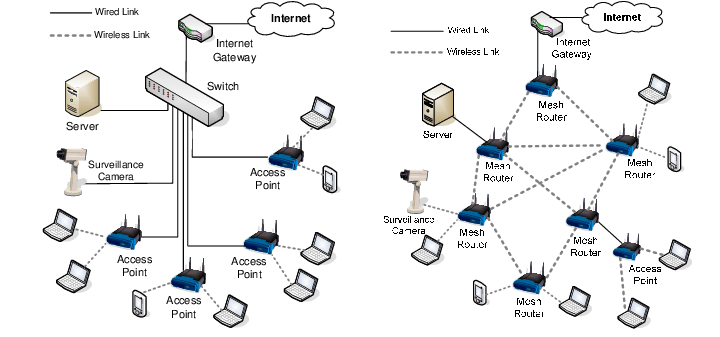
\includegraphics[scale=0.6]{Pictures/80211s.png}
	\caption{A comparison of 802.11 wlan and 802.11s mesh networks}
	\label{fig: 802.11s}
	\captionsetup{font={footnotesize,bf,it}}
	\caption*{source: Portmann, Marius. (2006). Wireless Mesh Networks for Public Safety and Disaster Recovery Applications. 10.1201/9781420013542.ch16. }
\end{figure}

\subsection{Routing in 802.11s}
Though there are a lot of routing protocols proposed in wireless mesh networks, the field is still active in research. What routing protocol to use closely depends on the application, and choice of the routing protocol may significantly impact the performance of the system. Different routing protocols can be mainly categorized into two types.

\begin{itemize}
	\item{\textbf{\textit{Proactive Routing Protocols:}} Proactive routing protocols are those protocols where the nodes keep track of the routes of all the accessible nodes. This is typically done by storing tables of all the routes based on the topology of the network. The tables are updated as the topology changes. While transmitting data, the node can instantly find the next hop from the routing table, which allows little or no latency in the sytem. On the other hand, to keep the tables updated with the topology , a lot of messages have to be sent between the nodes, which decreases the effective bandwidth for data. Moreover, these protocols tend to be slow to adapt to fast changes in topology. Some of the popular proactive routing protocols include \textit{Optimized Link State Routing} (OLSR) \cite{olsr}, \textit{Destination Sequenced Distance Vector} (DSDV) \cite{dsdv}, \textit{Better Approach To Mobile Adhoc Networking} (BATMAN) \cite{batman}, to name a few. }

	\item{\textbf{\textit{Reactive Routing Protocols:}} Where proactive routing protocols keep track of the routes based on topology, reactive routing protocols are on-demand routing protocols where a route between two nodes is found only when there needs to be communication between them. These protocols are defined to address the bandwidth issues of the proactive protocols. As they don't need to keep track of the routes, periodic flooding the network with messages to find the current topology, is not needed, which saves the bandwidth. On the other hand, these protocols tend to introduce more latency into the system as a route to a node has to be found before transmission of data. Some of the reactive routing protocols include \textit{Dynamic Source Routing} (DSR) \cite{dsr}, \textit{Adhoc On Demand Distance Vector} (AODV) \cite{aodv}. }
\end{itemize}

Due to significant research in routing protocols for mobile adhoc networks, there have been other classes of protocols as well, apart from the two main categories above. There are \textit{Hybrid Routing protocols}  like \textit{Zone Routing Protocol} (ZRP) \cite{zrp} and \textit{Temporarily Ordered Routing Algorithm} (TORA) \cite{tora}, which try to blend both low latency and bandwidth efficiency of proactive and reactive protocols together. There are also a class of \textit{Geographic Routing protocols} \cite{130, 131, 132} which are based on the geographic positions of the nodes, like GPS data for instance.

The 802.11s standard defines a mandatory default routing scheme called \textit{Hybrid Wireless Mesh Protocol} (HWMP), which is a hybrid protocol combining procative and reactive ascpects of routing protocols. However, it is not mandatory that one has to use the default HWMP and can implement any routing protocol while using 802.11s PHY and MAC layers.

\subsection{open80211s}
open80211s stack is an open source implementation of the 802.11s standard on the Linux kernel. It is based on mac80211 wireless stack, which implements the standard 802.11 on Linux kernel. Since it is based on mac80211 and makes minimal changes to the 802.11 MAC layer, it is supported on all legacy hardware that supports mac80211.

\begin{figure}
	\centering
	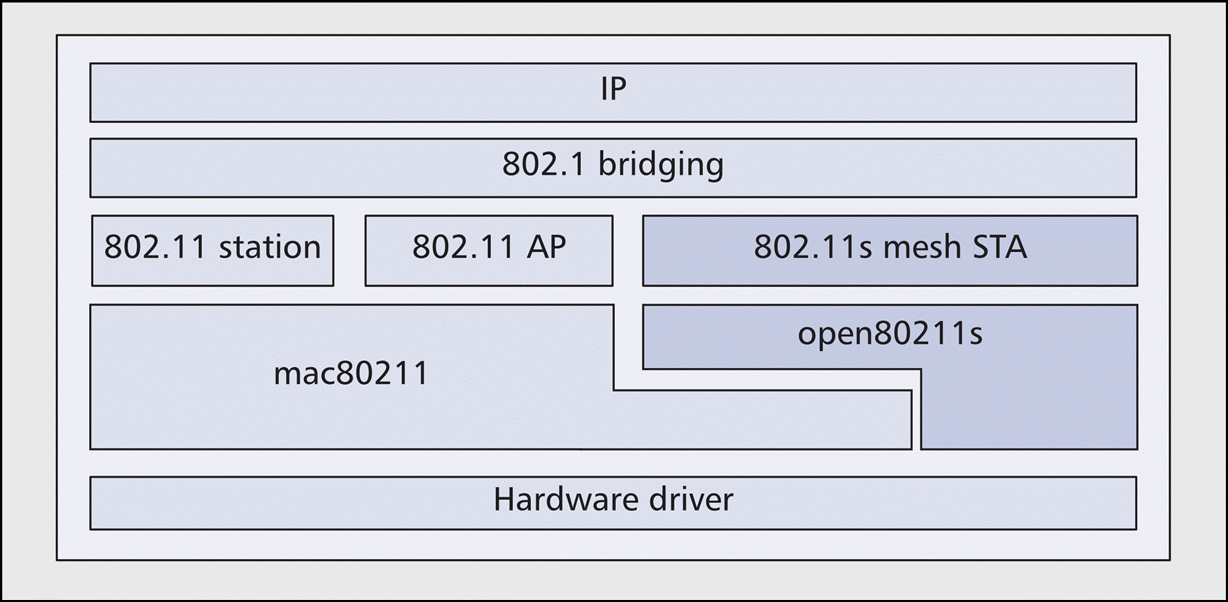
\includegraphics[scale=0.3]{Pictures/open80211s.png}
	\caption{open80211s stack on Linux kernel}
	\label{fig: open80211s}
	\captionsetup{font={footnotesize,bf,it}}
	\caption*{source: G. R. Hiertz et al., "IEEE 802.11s: The WLAN Mesh Standard," in IEEE Wireless Communications, February 2010.}
\end{figure}

\section{Hardware}
In this section, we shall look at the hardware used for realizing an 802.11s mesh network. As we mentioned in the last section, the open80211s stack can be implemented on most linux machines with legacy wireless cards which are compatible with the standard mac80211 wireless stack. There is a lack of embedded wireless hardware for building 802.11s mesh networks. We wanted to build 802.11s mesh networks with easily available commercial 802.11 legacy hardware and we found a solution with OpenWrt.

\begin{figure}
	\centering
	
\includegraphics[scale=1]{Pictures/openwrt_logo.jpg}
	\caption{logo of OpenWrt}
	\label{fig: openwrt}
	\captionsetup{font={footnotesize,bf,it}}
	\caption*{source: https://openwrt.org/}
\end{figure}

\subsection{OpenWrt}
Openwrt is an embedded operating system based on linux kernel, meant for wireless routers. Basically, it is an open source project in which the community releases ports of the operating system for specific wireless routers, whose wireless hardware is compatible and whose memory and firmware allow reflashing the default firmware, these devices come with. Since, not all wireless routers can be flashed with openwrt, we would have to choose from a list of openwrt compatible hardware.

Once we obtain an openwrt compatible wireless router, we would have to flash the router with an image of the openwrt operating system. Typically, different routers have different instructions for flashing the image and are generally listed along with other details on the device page, specific to the router. Once the router is flashed with openwrt, the device will be running a full-fledged operating system based on linux kernel, albeit one with limited capabilities. When we power on the router, it boots up into openwrt with a default ip address of 192.168.1.1/24. If we connect the router to a host machine via ethernet and \textit{ssh} into the said ip address, we would log into the openwrt with a secure shell.






